\documentclass[tikz,border=5mm]{standalone}
\usepackage[utf8]{vietnam}
\usepackage{tikz}
\usetikzlibrary{calc}
%=============
\begin{document}
	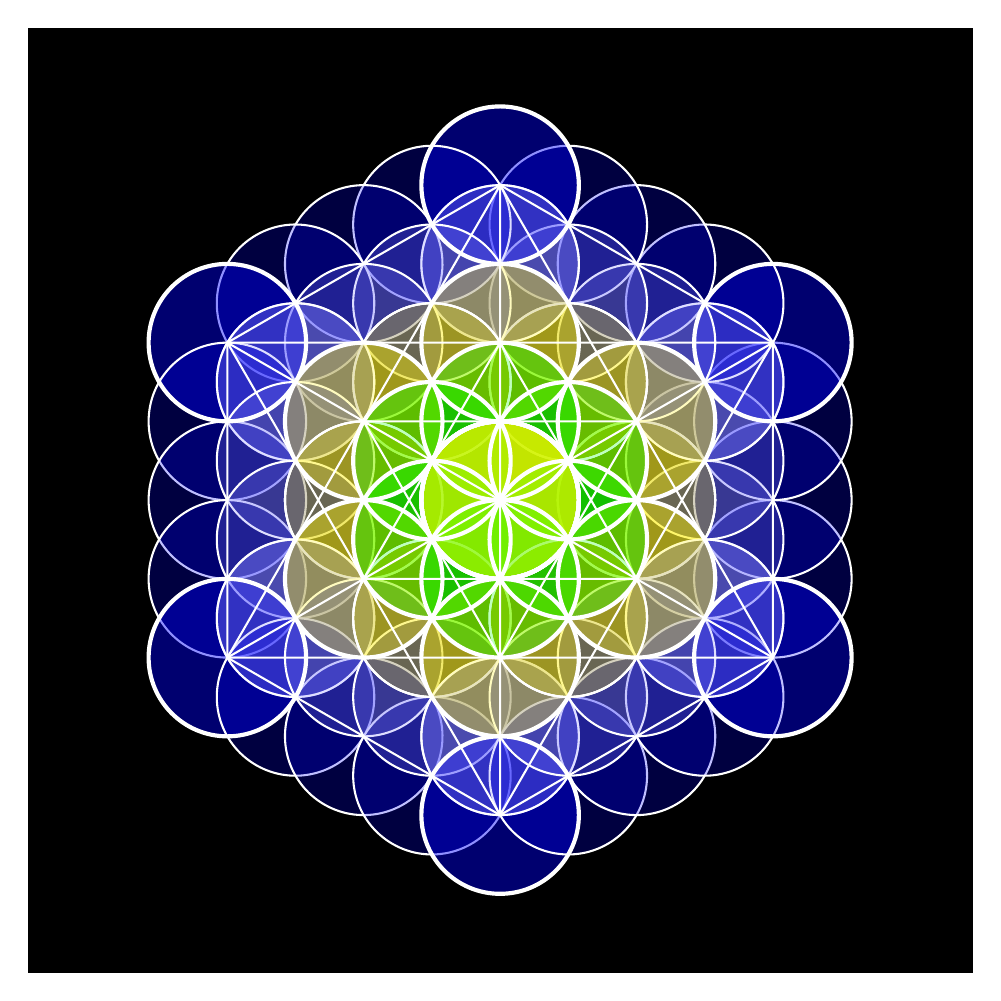
\begin{tikzpicture}[line width=0.75]
		\def\r{1}
		\pgfmathsetmacro{\rx}{\r *cos(30)}
		\pgfmathsetmacro{\ry}{\r *sin(30)}
		\fill[black](-6*\r,-6*\r) rectangle (6*\r,6*\r);
		%\fill[inner color=orange,outer color=black](0:0) circle (4*\r);
		\foreach \i in {0,60,...,300}{
			\foreach \j in {-4*\ry,-2*\ry,0,2*\ry,4*\ry}{
				\fill[rotate=\i,blue,opacity=0.25] (4*\rx,\j) circle (\r);
				\draw[white,rotate=\i] (4*\rx,\j) circle (\r);
			} %Vòng ngoài cùng (Vòng 1)
			\foreach \k in {-3*\ry,-\ry,\ry,3*\ry}{
				\fill[rotate=\i, blue!50,opacity=0.25] (3*\rx,\k) circle (\r);
				\draw[white,rotate=\i] (3*\rx,\k) circle (\r);
			}%Vòng tiếp theo (Vòng 2)
			\foreach \l in {-2*\ry,0,2*\ry}{
				\fill[rotate=\i ,yellow,opacity=0.25] (2*\rx,\l) circle (\r);
				\draw[white,rotate=\i ] (2*\rx,0) circle (\r);
			}
			\foreach \m in {-\ry,\ry}{
				\fill[rotate=\i ,green,opacity=0.25](\rx,\m) circle (\r);
				\draw[white,rotate=\i ](\rx,\m) circle (\r);
			}
			\fill[rotate=\i ,yellow,opacity=0.25](0,0) circle (\r);
			\draw[white,rotate=\i](0,0) circle (\r);
		}
		\foreach \i in {30,90,...,330}{\draw[white,line width=1.5] (\i:\r) circle (\r) (\i:2 *\r) circle (\r) (\i:4*\r) circle (\r) (0:0)circle(\r);}
		\draw [white,line width=1.5,opacity=0.25] (0:0) circle (\r);
		\draw[white] (30:4*\r)--(150:4*\r)--(270:4*\r)--cycle (30:2*\r)--(150:2*\r)--(270:2*\r)--cycle (30:4*\r)--(210:4*\r) (90:4*\r)--(270:4*\r) (150:4*\r)--(330:4*\r);
		\draw[white,yscale=-1] (30:4*\r)--(150:4*\r)--(270:4*\r)--cycle (30:2*\r)--(150:2*\r)--(270:2*\r)--cycle;
		\draw[white] (30:4*\r)--(90:4*\r)--(150:4*\r)--(210:4*\r)--(270:4*\r)--(330:4*\r)--cycle;
	\end{tikzpicture}
	%============
\end{document}